% ||||||||||||||||||||||||||||||||||||||||||||||
% Capitulo de Metodologia
% ||||||||||||||||||||||||||||||||||||||||||||||

\chapter{Metodologia}

O presente capítulo descreve todas as etapas do desenvolvimento do projeto, começando pela configuração do simulador de falhas MFS 
\textsuperscript \textregistered, da empresa SpectraQuest \textsuperscript \textregistered, até a implementação em campo. A metodologia do
desenvolvimento se encontra na figura \ref{fig:metodologia}, onde as etapas estão descritas em forma de fluxo de trabalho.

\begin{figure}[H]
    \caption{Metodologia do Projeto}
    \begin{center}
        \includegraphics[scale=1.1, page=3]{metodologia/img/software.pdf}
    \end{center}
    \fonte{Elaborado pelo autor.} 
    \label{fig:metodologia}
\end{figure}

Dentre as etapas descritas na imagem anterior, a simulação, o desenvolvimento do software, a integração do software com o hardware e a implementação
estão descritas com detalhes nos subcapítulos a seguir.


%++++++++++++++++++++++++++++++++++++++++++++++++++++++++++++++++
% 
%++++++++++++++++++++++++++++++++++++++++++++++++++++++++++++++++

\section{Configurações das Simulações}

Como dito anteriormente no fluxo de desenvolvimento, fez se o uso de simulações antes da implementação do sistema.
Para isso, foi utilizado um simulador de falhas em motores elétricos de indução e sistemas mancalizados, denominado
MFS \textsuperscript \textregistered (\textit{Machinery Fault Simulator} - simulador de falhas em máquinas), que pode ser visto na figura 
\ref{fig:real_plant}. O simulador é composto por um motor elétrico de indução trifásico de 1 HP, o qual está conectado com um eixo via um 
acoplamento. Esse eixo possui dois discos dourados e furados, onde é possível se colocar cargas para criar um desbalanceamento no sistema.

\begin{figure}[H]
    \caption{Estrutura do simulador MFS \textsuperscript \textregistered.}
    \begin{center}
        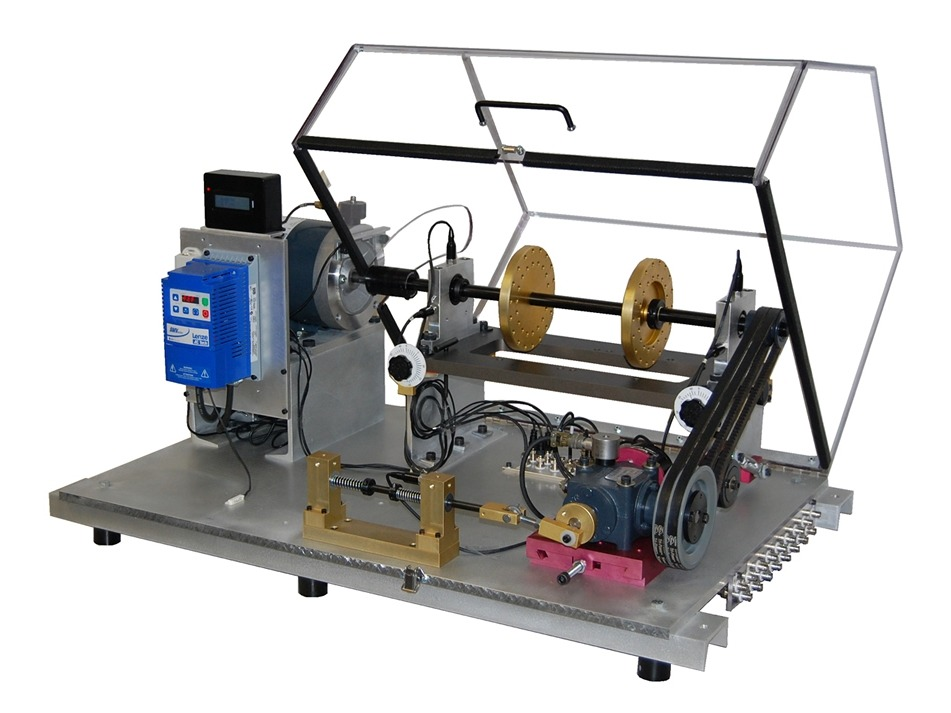
\includegraphics[scale=.4]{metodologia/img/real_plant.jpeg}
    \end{center}
    \fonte{\citeonline{SpectraQuest2011}.} 
    \label{fig:real_plant}
\end{figure}

Para a realização dos testes, diversas combinações de falhas, frequências do inversor e frequências de amostragem foram
utilizadas, para se entender as dinâmicas das falhas em diferentes condições de testes. A planta possui diversos acelerômetros e um sensor
de corrente, que está amostra uma das fases da alimentação. As falhas que foram inseridas nos testes foram: desalinhamento dos
mancais e o desbalanceamento das cargas. Essas partes podem ser vistas na figura \ref{fig:lateral_desenho}.

\begin{figure}[H]
    \caption{Desenho simplificado da Planta.}
    \begin{center}
        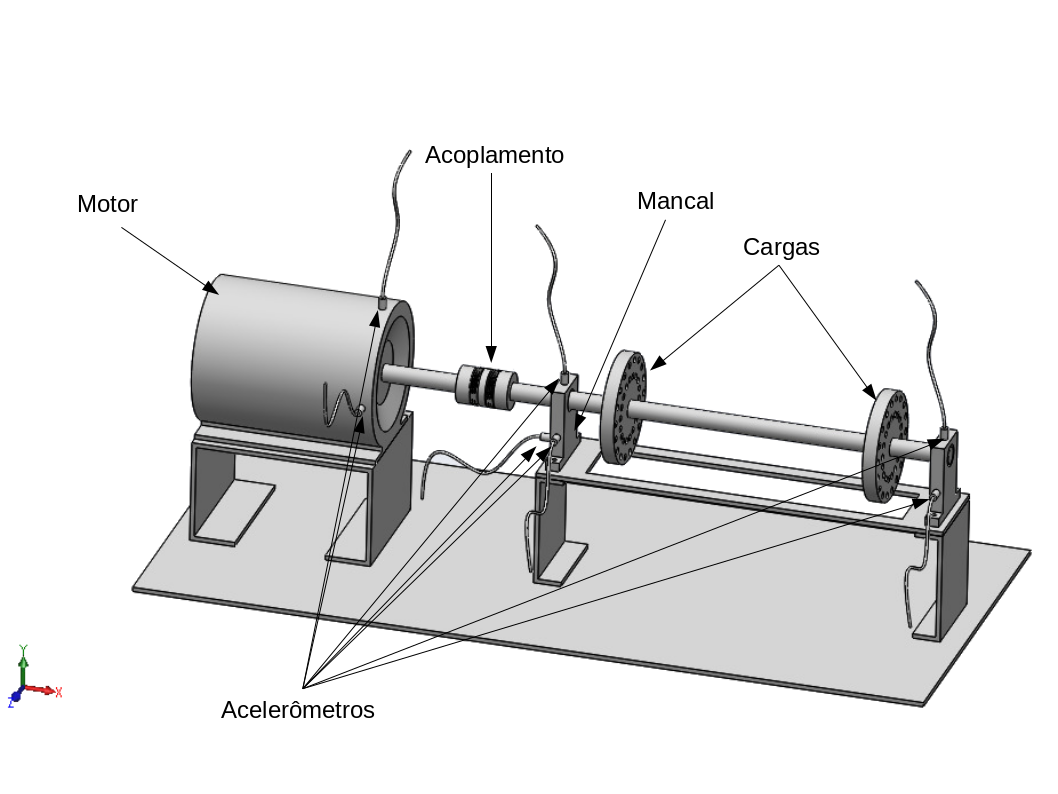
\includegraphics[scale=.5]{metodologia/img/lateral_desenho.png}
    \end{center}
    \fonte{Elaborado pelo Autor.} 
    \label{fig:lateral_desenho}
\end{figure}

A tabela \ref{tab:simulador} contem as combinações de testes que foram realizados. Onde DA é desalinhamento e DB é desbalanceamento.
Cada um destes arquivos gerados possuem 9 colunas de dados, que correspondem aos 7 acelerômetros, 1 tacógrafo e um transformador de
corrente.

\begin{table}[H]
    \caption{Testes realizados.}
    \label{tab:simulador}
    \centering%
    \begin{minipage}{\textwidth}
      \begin{tabular*}{\textwidth}{cccc}
        \hline
        {Nome}                   & Falha                     & Freq. do motor [Hz] & Amostragem [kHz]\\ \hline
        \hline
        Bom                      &  Sem                      &      60             &    25  \\ 
        Misa15                   &  DA de 15 mils            &      60             &    10  \\
        Misa35\_10k\_20Hz        &  DA de 35 mils            &      20             &    25  \\
        Misa35\_10k\_20Hz\_unb   &  DA de 35 mils e DB       &      20             &    25  \\
        Misa35\_10k\_30Hz\_unb   &  DA de 35 mils e DB       &      30             &    25  \\
        Misa35\_10k\_40Hz        &  DA de 35 mils            &      40             &    25  \\
        Misa35\_10k\_5Hz         &  DA de 35 mils            &      5              &    25  \\
        Misa35\_10k\_80Hz        &  DA de 35 mils            &      80             &    25  \\
        Misa35\_8k               &  DA de 35 mils            &      20             &    20  \\ \hline
      \end{tabular*}
      \fonte{Elaborado pelo Autor.} 
    \end{minipage}
  \end{table}
  
Após a apresentação de como foram realizados os testes no simulador, é possível aplicar as topologias propostas no presente trabalho nos
dados gerados. Após a etapa de simulação e análise dos dados, com os resultados obtidos, foi possível o início do desenvolvimento do software,
que será descrito na próxima etapa. 


%++++++++++++++++++++++++++++++++++++++++++++++++++++++++++++++++
% 
%++++++++++++++++++++++++++++++++++++++++++++++++++++++++++++++++

\section{Desenvolvimento do Software}

Com a escrita dos requisitos, simulações e análise dos dados das simulações, foi possível o início da etapa de desenvolvimento de software,
que agrega várias ferramentas para entregar um sistema de tempo real para o monitoramento da saúde de motores elétricos de indução. A 
implementação foi dividida em três principais tarefas: aquisição dos dados, machine learning e o monitoramento. As duas primeiras estão
descritas na imagem a seguir.

\begin{figure}[H]
    \caption{Tarefas de Aquisição e Machine Learning}
    \begin{center}
        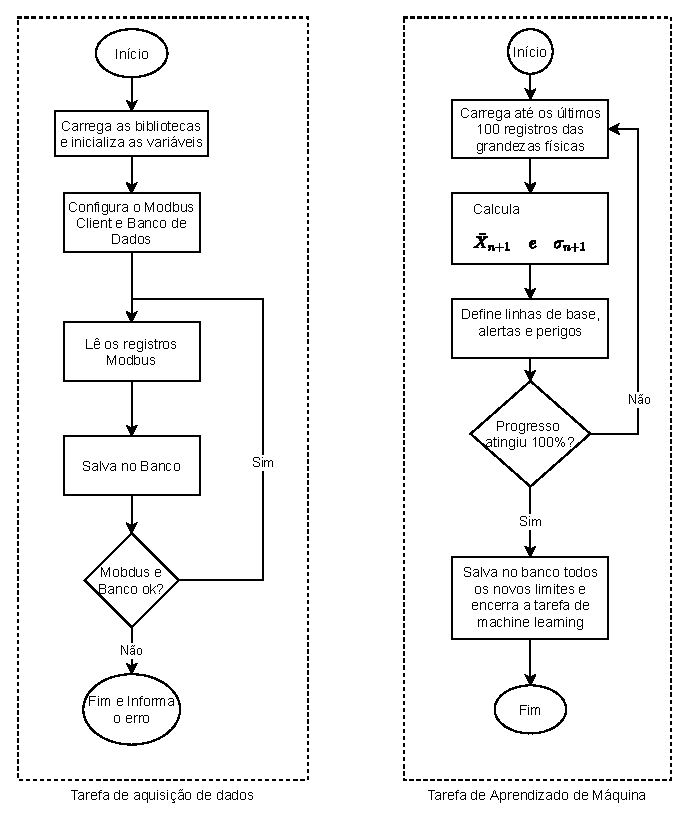
\includegraphics[scale=1, page=1]{metodologia/img/software.pdf}
    \end{center}
    \fonte{Elaborado pelo autor.} 
    \label{fig:tarefa_aq_ml}
\end{figure}

Na tarefa de aquisição de dados, a qual foi desenvolvida utilizando a linguagem de programação Python, o protocolo utilizado foi o Modbus, 
muito comum na indústria e de fácil utilização, principalmente porque a leitura é feita de forma periódica e com um intervalo de até 
\SI{5}{\minute} entre cada uma, que é um dos conceitos básicos do protocolo. O banco de dados utilizado é o InfluxDB, um baco de dados não 
relacional para armazenamento de séries temporais, que também é uma característica dos dados amostrados.
Já na tarefa de aprendizado de máquina, ela  manipula banco de dados e variáveis de ambiente da aplicação para encontrar as linhas de base e
os limiares de alerta e perigo, basicamente encontrando as seguintes relações:

\begin{equation}\label{eq:ml}
    \bar{X}_{n+1} = \bar{X}_{n} + \frac{x + \bar{X}_n}{n}
\end{equation}

Onde $\bar{X}_{n+1}$ é a média aritmética para os $n+1$ elementos, $ \bar{X}_{n}$ é a média aritmética anterior,
$x$ é o novo dado adquirido. Já a relação da variância, pode ser calculada da seguinte forma:


\begin{equation}\label{eq:ml2}
    n \cdot var_{n+1} = var_{n} + (x - \bar{X}_{n+1})(x-\bar{X}_n)
\end{equation}

E por fim, o desvio padrão $\sigma_{n+1}$ para um novo elemento:
\begin{equation}\label{eq:ml3}
    \sigma_{n+1} = \sqrt{\frac{var}{n}}
\end{equation}

Assumimos que a região de alerta ($A$), a qual significa uma moderada tendência à falha, pode ser calculada da seguinte forma: 
\begin{equation}\label{eq:ml4}
    A = \bar{X}_{n+1} + 2 \sigma
\end{equation}

Segundo a mesma regra, a região onde há uma falha iminente ($P$), um comportamento ambiental ou regime de funcionamento atípico, 
pode ser calculado da seguinte forma:

\begin{equation}\label{eq:ml5}
    P = \bar{X}_{n+1} + 3 \sigma
\end{equation}

Após os valores das linhas de base, alerta e perigo, a aplicação pode ficar encarregada de monitorar os novos dados e aplicar um conjunto
de regras para classificar se o motor elétrico de indução tem um comportamento normal. O fluxograma da sequência descreve tal tarefa.

\begin{figure}[H]
    \caption{Tarefa de monitoramento}
    \begin{center}
        \includegraphics[scale=1, page=2]{metodologia/img/software.pdf}
    \end{center}
    \fonte{Elaborado pelo autor.} 
    \label{fig:monitoramento}
\end{figure}

Os critérios elencados para se decidir sinalizar uma tendência de falhas, como podem ser vistos no fluxograma anterior, pode ser divididos
em duas partes. A primeira, para evitar que dados espúrios ou alguma vibração atípica interfira no sistema, somente se 5 amostras apresentarem 
valores maiores ou iguais aos limites um sinal de alerta, ou perigo, um sinal será gerado. No segundo caso, se a média dos últimos 100 elementos
for maior, eliminando os casos em que o motor pode ter um regime não contínuo dentro das 5 amostras, tendo apenas 4 ou menos amostras com valores
excedentes.

Para uma interface entre homem e máquina, utilizamos a ferramenta Node-Red parta prototipar a presente aplicação. A imagem da sequência mostra 
a estrutura básica das telas do sofware, que é uma ferramenta baseada em web que pode ser acessada por qualquer dispositivo com navegador web que esteja
na rede.

\begin{figure}[H]
    \caption{Fluxo de acesso do Software.}
    \begin{center}
        \includegraphics[scale=0.8, page=2]{metodologia/img/fluxo_layout.pdf}
    \end{center}
    \fonte{Elaborado pelo autor.} 
    \label{fig:fluxo_software}
\end{figure}

Como vemos, a aplicação possui uma tela de login que protege o acesso ao dashboard principal, que contém imagens que facilitam a identificação
visual de algum problema com o motor ou com o sistema de aquisição de dados. Ao se selecionar um dos motores, a aplicação é redirecionada para
uma tela que contém um grupo de gráfico e configurações. A aplicação também permite a configuração manual dos limites de alerta e perigo.
Após a conclusão e aprovação do software, foi possível executar a integração entre hardware e software, para finalizar o desenvolvimento. Esta
etapa está descrita na sequência.

%++++++++++++++++++++++++++++++++++++++++++++++++++++++++++++++++
% 
%++++++++++++++++++++++++++++++++++++++++++++++++++++++++++++++++

\section{Integração entre Software e Hardware}

Para a aquisição das grandezas físicas, as quais alimentam a aplicação de software, foi selecionado o sensor de vibração e temperatura QM30VT2, 
da Banner Engineering, que possui as seguintes característica:

\begin{table}[H]
    \caption{Especificações do Sensor QM30VT2}
    \label{tab:espec_sensor}
    \centering%
    \begin{minipage}{.45\textwidth}
      \begin{tabular*}{\textwidth}{c|c}
        \hline
        Especificação            & Valores                                     \\ \hline
        \hline
        Intervalo de medição     &  0 a $\SI{46}{\milli\metre\per\second}$     \\
        Largura de banda         &  10 a $\SI{4}{\kilo\hertz}$                 \\ 
        Acurácia                 &  $\mp 10 \%$ a $\SI{25}{\celsius}$          \\
        Amostragem               &  $\SI{20}{\kilo\hertz}$                     \\
        Tempo de Amostragem      &  $\SI{0.4}{\second}$                        \\
        Grau de Certificação     &  IP67                                       \\ \hline
      \end{tabular*}
      \fonte{Elaborado pelo Autor.} 
    \end{minipage}
  \end{table}

Como podemos ver, ele possui uma largura de banda de até $\SI{4}{\kilo\hertz}$, propícia até para detecção de falhas em rolamentos, como 
descrito no referencial teórico. Os dados são adquiridos via Modbus RTU (\textit{Remote Terminal Unit} - Unidade de terminal remoto) diretamente
do sendor, ou ainda, via Modbus TCP (\textit{Transmission Control Protocol} - Protocolo de Controle de Transmissão) a partir de um gateway
wireless e um nó, facilitando a implantação por não utilizar cabos entre os sensores e a unidade de processamento. O diagrama da figura a seguir
representa o fluxo básico dos sinais, indo do sensor até o sistema embarcado, o qual processa, armazena e disponibiliza a visualização em 
tempo real dos dados. 

\begin{figure}[H]
    \caption{Diagrama de integração  entre sensores e Software.}
    \begin{center}
        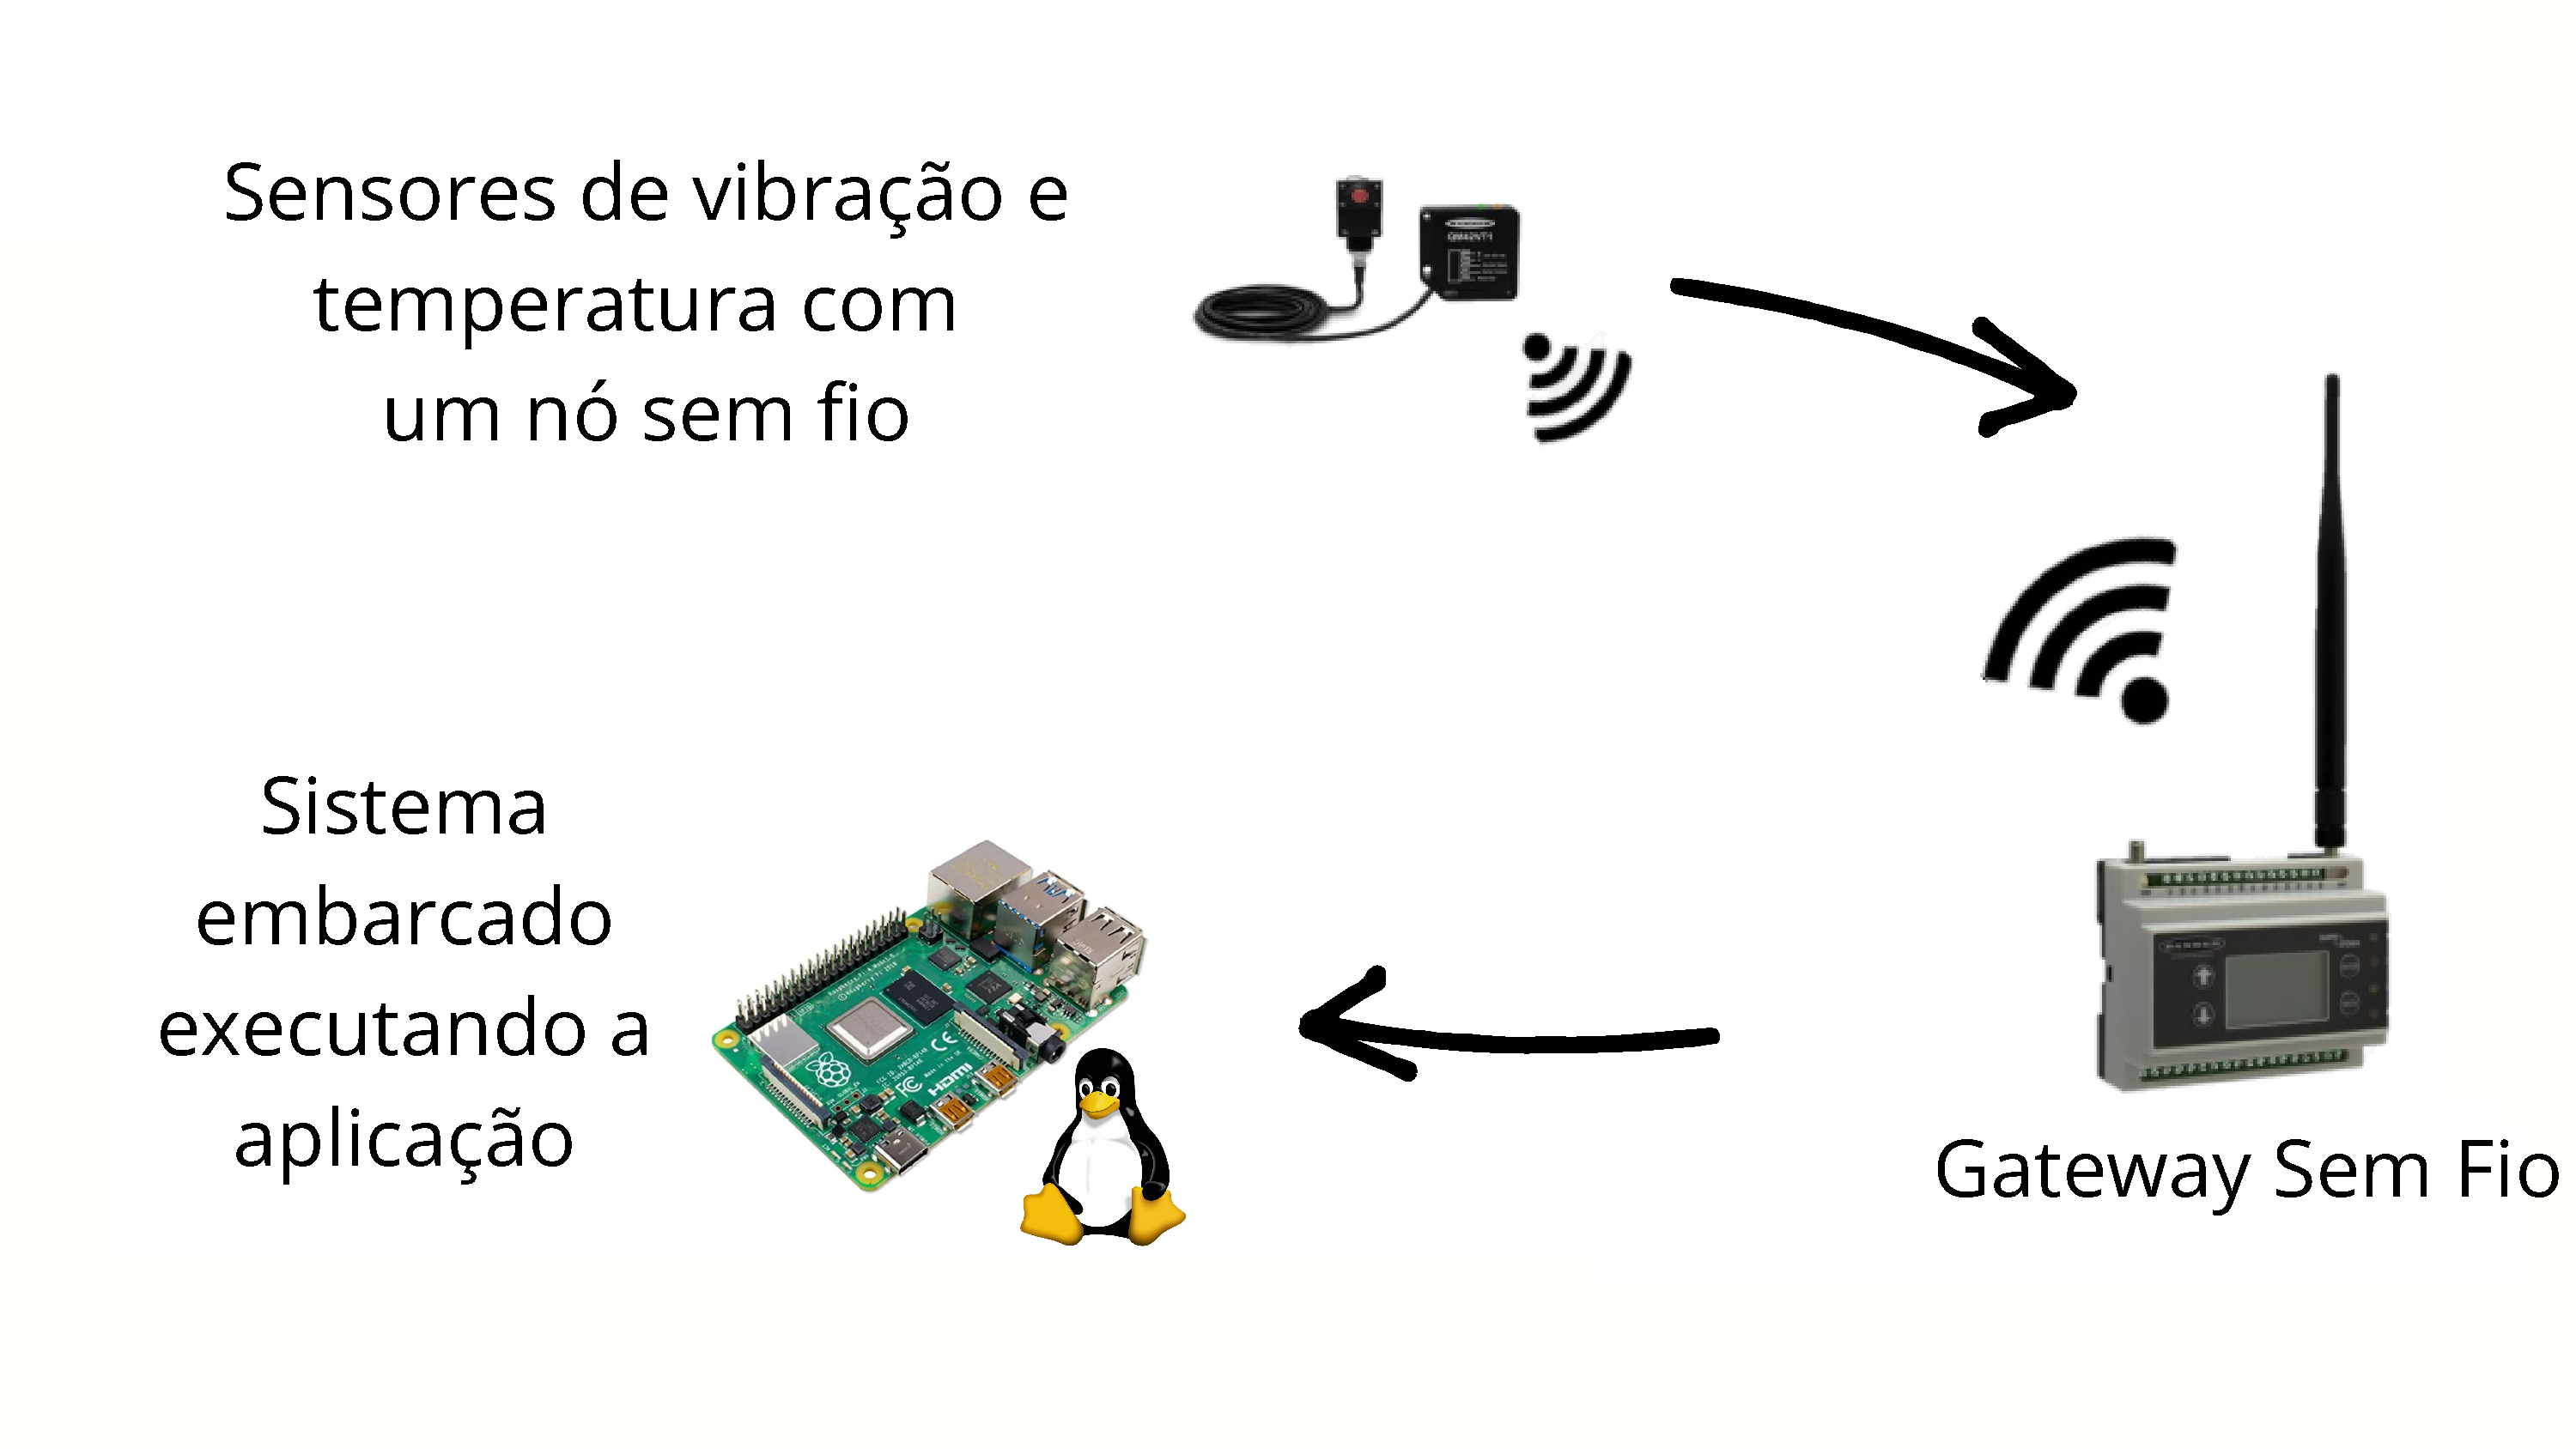
\includegraphics[scale=0.8, page=1]{metodologia/img/fluxo_layout.pdf}
    \end{center}
    \fonte{Adaptado pelo autor.} 
    \label{fig:fluxo_integracao}
\end{figure}


O sistema embarcado, o qual é a unidade de processamento da aplicação, é composto por uma Raspberry Pi 3 Modelo B+, que é um dispositivo muito 
conhecido e confiável, executando uma distribuição Linux baseada em Debian. Após o desenvolvimento de software, da integração com o hardware, 
prototipação, o projeto foi executado em campo, em forma de estudo de caso, em uma empresa da região metropolitana de Porto Alegre - RS, seguindo o fluxograma da 
figura \ref{fig:metodologia}, que será descrito na próxima etapa.

%++++++++++++++++++++++++++++++++++++++++++++++++++++++++++++++++
% 
%++++++++++++++++++++++++++++++++++++++++++++++++++++++++++++++++

\section{Estudos de Casos}


Como descrito no fluxograma do projeto, a etapa final do desenvolvimento é a de testes em campo, em forma de estudo de caso, com o objetivo 
de analisar a robustez do produto, da comunicação entre o sensor e a unidade de processamento e da confiabilidade da aplicação de software. 
Para aplicar a solução, foram escolhidos equipamentos reais e funcionais, que operam 24 horas, 7 dias por semana em empresas parceiras,
com o objetivo de prova de conceito e posterior aquisição pelas mesmas. Para isto, um exaustor industrial foi escolhido em uma delas, que é 
uma montadora da região metropolitana de Porto Alegre - RS. A figura \ref{fig:exautor} representa um exaustor industrial, um dispositivo que com o decorrer do uso, apresenta severas falhas com o acumulo 
de partículas que estão suspensas no ar. Uma falha num dispositivo como este, acarreta uma parada de  produção, impactando diretamente no 
financeiro da empresa, justificando facilmente o investimento da tecnologia desenvolvida neste trabalho.

\begin{figure}[H]
    \caption{Fotografia externa de um exaustor industrial.}
    \begin{center}
        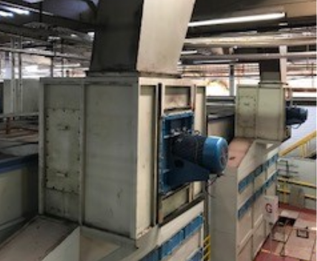
\includegraphics[scale=1.25]{metodologia/img/exaustor.png}
    \end{center}
    \fonte{Fornececida pela empresa.} 
    \label{fig:exautor}
\end{figure}

Em um destes dispositivos, foi instalado um sensor industrial de vibração e temperatura, com o objetivo de coletar, processar e armazenar os
dados, criando um dashboard com o estado de saúde do motor elétrico de indução. A figura \ref{fig:sensor_exaustor} apresenta o sensor instalado.
O motor já se encontrava em uso há algum tempo antes dos testes em campo, significando que já existe uma base de vibração maior do que se fosse
um motor há pouco recondicionado, exigindo um ajuste manual na ferramenta de machine learning, reduzindo os limites criados pelo software, que
consideram que o motor está em perfeito estado de saúde para começar a criação dos limites. Já estava previsto na etapa de análise de mercado, 
a possibilidade de se ajustar os resultados do machine learning, devido a grande frequência de instalações em motores que possuem médio ou
elevado MTBF (\textit{mean time between failures} - tempo médio entre falhas), mas que ainda oferecem prejuízos se a falha acorrer de forma 
imprevista.

\begin{figure}[H]
    \caption{Fotografia externa do sensor instalado em um exaustor industrial.}
    \begin{center}
        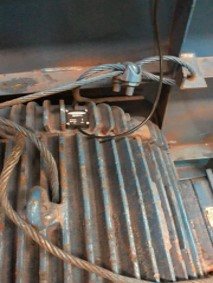
\includegraphics[scale=1.1]{metodologia/img/sensor_exaustor.jpg}
    \end{center}
    \fonte{Forncecida pela empresa.} 
    \label{fig:sensor_exaustor}
\end{figure}

Já as características dos testes, que podem ser vistas na tabela \ref{tab:exautor}, 

\begin{table}[H]
    \caption{Características da prova de conceito no exaustor}
    \label{tab:exautor}
    \centering%
    \begin{minipage}{.55\textwidth}
      \begin{tabular*}{\textwidth}{c|c}
        \hline
        Característica                          & Valores                                    \\ \hline
        \hline
        Tempo entre cada amostragem             &  $\SI{5}{\minute}$                         \\
        Número de sensores                      &  1                                         \\ 
        Potência do motor                       &  yyyy$\SI{}{\kilo\watt}$                      \\
        Classe do motor segundo a  ISO 10816-1  &  I                                         \\
      \end{tabular*}
      \fonte{Elaborado pelo Autor.} 
    \end{minipage}
  \end{table}


Já na outra empresa, que é uma produtora de tabaco e seus derivados, também no estado do Rio grande do sul, o sistema foi instalado em uma 
seleira universal, não especificamente em um motor elétrico de indução, mas em 5 pontos estratégicos, distribuindo os 5 sensores nos principais pontos 
de falhas: acoplamentos, moto-redutores e nas proximidades de polias. Esta seleira universal tem um papel muito importante na produção, sendo um dos gargalos
da produção. Qualquer falha imprevista, também impacta na produção diária, distorcendo toda a produção. A tabela \ref{tab:seleira_universal} apresenta 
as características da prova de conceito na seleira universal.

\begin{table}[H]
    \caption{Características da prova de conceito na seleira universal}
    \label{tab:seleira_universal}
    \centering%
    \begin{minipage}{.55\textwidth}
      \begin{tabular*}{\textwidth}{c|c}
        \hline
        Característica                          & Valores                                    \\ \hline
        \hline
        Tempo entre cada amostragem             &  $\SI{30}{\second}$                        \\
        Número de sensores                      &  5                                         \\ 
        Potência do motor                       &  $\SI{1.1185}{\kilo\watt}$                 \\
        Classe do motor segundo a  ISO 10816-1  &  I                                         \\
      \end{tabular*}
      \fonte{Elaborado pelo Autor.} 
    \end{minipage}
  \end{table}

Como podemos ver, a amostragem e o número de sensores são as principais diferenças. A amostragem com 10 vezes mais elementos, foi uma exigência
da empresa, além do mais, o equipamento tem variações de ciclos, não sendo um processo contínuo, inviabilizando amostras com intervalo de 
$\SI{5}{\minute}$. Imagens da instalação dos sensores, e nem da máquina, foram liberadas pela empresa, mas os resultados foram 
disponibilizados na íntegra.

Após a descrição de toda a metodologia do presente trabalho, iniciando pela estrutura básica da metodologia, das simulações, do desenvolvimento
do software, da integração de software e hardware, e por fim, a instalação do protótipo nas empresas parceiras, para a prova de conceito, 
podemos apresentar os resultados, que se encontram no próximo capítulo.